\chapterformat{Simulation}

In this chapter we describe the implementation of the numerical simulation used to model the behavior of the EMILIE membrane. The focus is on the assumptions underlying the model, the construction of the computational domain and material parameters, and the algorithms employed for solving the eigenvalue problem. Particular attention is given to the treatment of perforations, electrodes, and sampled masses, as well as to numerical aspects such as mesh convergence, preconditioning, mode detection, and stability of the solver. Together, these components establish a simulation framework that can be directly compared to experimental measurements and adapted to different device configurations. An image of both the membrane and the mesh are given in Figure \ref{fig:mesh}.\\

\section{Assumptions}
\label{sec:assumptions}
The following assumptions underlie the simulation: 
\begin{itemize}
    \item The membrane is modeled in two spatial dimensions.
    \item The bending stiffness of the membrane is negligible. This assumption is analytically justified in section \ref{sec:bending_stiffness}.
    \item A linear mechanical regime is assumed. The displacements on the membrane are sufficiently small for the material response to remain within the linear elastic range.
    \item For the forward coupling of the two PDEs, it is assumed that the membrane deformations due to vibrations are small enough that they do not significantly alter the prestress.
    \item The perforation is modeled as a continuous part of the membrane with effective density and prestress values.
\end{itemize}

\subsection{Influence of the bending stiffness}
\label{sec:bending_stiffness}
In this section, an analytical argument is given that shows that the bending stiffness of the membrane can be neglected. Consider a homogeneous square membrane without additional features. In the equation of motion, the force contribution from the prestress is $\sigma \nabla^2 u$, whereas the contribution from bending stiffness is $D_p \nabla^4 u$, where $\sigma$ is the prestress and 
\[
D_p = \frac{E h^3}{1-\nu^2}
\]
is the flexural rigidity, with $E$ denoting the Young's modulus, $h$ the membrane thickness, and $\nu$ the Poisson ratio \cite{schmid2016fundamentals}. The governing PDE is
\begin{equation}
    \sigma \nabla^2 u + D_p \nabla^4 u - \frac{\partial^2 u}{\partial t^2} = 0.
    \label{eq:kirchhoff_wave}
\end{equation}

As shown in \cite{schmid2016fundamentals}, this PDE admits solutions of the form $u:\mathbb{R}^2\to\mathbb{R}$,
\begin{equation*}
    u(x,y,t) = u_0 \, \sin\!\left(\frac{n\pi}{L}x\right) \sin\!\left(\frac{j\pi}{L}y\right) 
    \cos(\omega_{ij} t),
\end{equation*}
with mode indices $n,j \in \mathbb{N}$, amplitude $u_0 \in \mathbb{R}$, and membrane side length $L = \SI{1}{\milli\meter}$.\\

Substituting this ansatz into equation \eqref{eq:kirchhoff_wave} and eliminating the trigonometric factors yields
\begin{equation}
    -\sigma \left[ \left(\frac{n\pi}{L}\right)^2 + \left(\frac{j\pi}{L}\right)^2 \right]
    + D_p \left[ \left(\frac{n\pi}{L}\right)^4 + 2 \left(\frac{n\pi}{L}\right)^2 \left(\frac{j\pi}{L}\right)^2 + \left(\frac{j\pi}{L}\right)^4 \right]
    + \rho h \, \omega_{ij}^2 = 0.
    \label{eq:eigeneq_analytical}
\end{equation}

We refer to the term containing $D_p$ as the \emph{bending term} and the term containing $\sigma$ as the \emph{prestress term}. Since the bending term involves the fourth powers of $n$ and $j$, while the membrane term involves only second powers, the influence of bending stiffness grows with increasing mode number. In the simulations, we consider only modes up to $(n,j) = (3,1)$. Thus, the $(3,1)$ mode is the most affected by bending stiffness.

Solving equation \eqref{eq:eigeneq_analytical} for $\omega_{31}$ using a prestress of $\sigma=\SI{25}{\mega\pascal}$ 
\[
\omega_{31} \approx \SI{9.1e5}{\per\second}.
\] 
Repeating the calculation while omitting the bending term yields 
\[
\omega_{31,\mathrm{nb}} \approx \SI{9.1e5}{\per\second}.
\] 
The relative difference is
\[
\frac{|\omega_{31} - \omega_{31,\mathrm{nb}}|}{\omega_{31}} \approx 5.4 \cdot 10^{-12}.
\]
The detailed calculations can be found in \texttt{analytical\_case.py}. This result shows that the bending stiffness is entirely negligible even in the highest considered modes with relatively small prestress, justifying its omission in the more complex case with electrodes and additional features.\\




\section{Domain Geometry}

In this section, we discuss the implementation of the two-dimensional membrane geometry in the simulation. The mesh used in most simulation runs is shown in Figure \ref{fig:mesh} (A) and is generated with the function \texttt{generate\_mesh}. Different meshes are only used in the convergence analysis (section \ref{sec:convergence_analysis}) and in studies of alternative membrane geometries (section \ref{sec:membrane_size}). Additionally, when a sample is placed on the membrane, the mesh is adapted to resolve this sample (see section \ref{sec:polypropylene} and Figure \ref{fig:other_modeshapes}).  

In the convergence analysis, only finer meshes are employed, since the mesh in Figure \ref{fig:mesh} (A) already represents the coarsest possible mesh that still resolves the electrodes. For alternative membrane geometries, the mesh changes accordingly; however, the mesh parameters (most importantly the element size and minimum angles) are chosen to remain comparable.\\



\begin{figure}[h]
    \centering
    \begin{overpic}[height=\domainheight,
    trim=2.2cm 2.2cm 2.2cm 2.2cm,
        clip]{figures/pngs/mesh.png}
        \put(15,70){\large\bfseries\textcolor{white}{A}}
    \end{overpic}%
    \hspace{1cm}
    \begin{overpic}[height=\domainheight]{figures/pngs/empty_membrane.png}
        \put(8,90){\large\bfseries\textcolor{white}{B}}
    \end{overpic}
    \caption{(\textbf{A}) Mesh for the simulation with default parameters and \SI{1}{\milli\meter} side length. The mesh resolves both the electrodes and the boundary of the perforated area. (\textbf{B}) Image of an unsampled membrane with \SI{1}{\milli\meter} side length.}
    \label{fig:mesh}
\end{figure}




\subsection{Electrode Geometry}
\label{sec:electrode_geometry}

We now describe the geometry of the electrodes and its implementation in the simulation.\\

The electrodes have a parabolic shape and are modeled as
\[
f(x) = a x^2 + b x + c.
\]
The perforation radius $R_\mathrm{perf}$ is treated as an open parameter in order to study its effect on the system. This leaves a free space of $L/2 - R_\mathrm{perf}$ for the electrodes. The maximum height of the parabola is parameterized by $P_\mathrm{el}$, defined as the fraction of this free space occupied by the electrodes. Accordingly, the maximum of $f$ is
\[
P_\mathrm{el} \cdot \bigl(L/2 - R_\mathrm{perf}\bigr).
\]
Solving for the parabola parameters yields
\[
a = -\frac{4 P_\mathrm{el} (L/2 - R_\mathrm{perf})}{L^2}, \quad 
b = -aL, \quad
c = w_e/2,
\]
where $w_e = 10\,\mu\mathrm{m}$ denotes the electrode width.\\

The left electrode occupies the region
\begin{equation}
    E_l = \left\{ (x,y) \in \mathbb{R}^2 : 
    a y^2 + b y + c - \tfrac{w_e}{2} < x < a y^2 + b y + c + \tfrac{w_e}{2} \right\},
    \label{eq:domain_left_electrode}
\end{equation}
and the right electrode is symmetrically placed,
\begin{equation}
    E_r = \left\{ (L-x,y) \in \mathbb{R}^2 : 
    a y^2 + b y + c - \tfrac{w_e}{2} < x < a y^2 + b y + c + \tfrac{w_e}{2} \right\},
    \label{eq:domain_right_electrode}
\end{equation}
where $L = \SI{1}{\milli\meter}$ is the side length of the membrane.\\

To implement the electrodes in the mesh, points on their boundaries $\partial E_l$ and $\partial E_r$ must be defined. Multiple layers of elements across the electrode width can optionally be included for parameter studies (although we later confirm that a single layer suffices). To minimize poor angles in the mesh elements, the boundary points are placed such that the connecting edge between corresponding vertices on both sides of the electrode is perpendicular to the face. This is achieved using the derivative
\[
f'(y) = 2 a y + b,
\]
so that for a given $y$, the boundary points are
\[
\bigl(f(y) + w_e/2,\, y + f'(y) \cdot w_e/2 \bigr), \quad
\bigl(f(y) - w_e/2,\, y - f'(y) \cdot w_e/2 \bigr).
\]
This construction is implemented in the function \texttt{points\_on\_parabola}.\\

For coefficient functions (density and prestress), the electrode geometry is represented as a function 
\[
g_\mathrm{el} : \mathbb{R}^2 \to \{0,1\}, \quad g_\mathrm{el}(\mathbf{x}) = 
\begin{cases}
1, & \mathbf{x} \in E,\\
0, & \text{otherwise}.
\end{cases}
\]
This is implemented in the functions \texttt{geom\_el\_parabola} and \texttt{geom\_el\_both}.\\

In the elasticity problem, the electrode geometry also enters through an additional prestress that produces a perpendicular force on the electrode faces. A unit vector perpendicular to the electrode boundaries can be constructed from the tangent vector
\[
\mathbf{v}_\parallel = 
\begin{pmatrix}
f'(y) \\ 1
\end{pmatrix}, 
\quad
\mathbf{v}_\perp = \frac{1}{\sqrt{1+(f'(y))^2}}
\begin{pmatrix}
1 \\ -f'(y)
\end{pmatrix}.
\] 
This is implemented in the function \texttt{force\_CF}.\\

\subsection{Perforation Geometry}

The perforation is modeled as a continuous region of the membrane (see section \ref{sec:definition_effective_parameters}). The membrane is meshed uniformly, but the perforation requires modified material parameters and interface boundary conditions on its boundary. Therefore, the perforation boundary is explicitly resolved in the mesh. Equidistant nodes are placed along the boundary and connected via labeled edges in the function \texttt{generate\_mesh}.\\

\section{Effective Parameters on the Membrane}
\label{sec:definition_effective_parameters}

We assume that the perforation can be modeled as a continuous part of the membrane with effective density and prestress. The effective density is reduced by the missing mass due to the holes. The holes have a radius of $r = \SI{2.97}{\micro\meter}$ and a rim-to-rim spacing of $r$, resulting in an effective density
\[
\rho_\mathrm{eff} = 0.62\, \rho_\silnit.
\]
with the membrane density $\rho_\silnit = \rho^{\mathrm{3D}}_\silnit h_\silnit$.
We further assume that the effective prestress on the perforated region remains unchanged,
\[
\sigma_\mathrm{eff} = \sigma_\silnit.
\]
This assumption is based on the heuristic that the original stress redistributes across the remaining material without significant change in the average prestress. This hypothesis will be tested in section \ref{sec:parameter_search}.  

For convenience, we introduce normalized parameters
\[
\rho_\mathrm{eff}^* = \frac{\rho_\mathrm{eff}}{\rho_\silnit}, \qquad
\sigma_\mathrm{eff}^* = \frac{\sigma_\mathrm{eff}}{\sigma_\silnit}.
\]

\section{Coefficient Functions}

The PDE formulations require several coefficient functions, specifically for the density, prestress, Young’s modulus, and Poisson ratio. These are implemented in the functions \texttt{generate\_rho\_fct}, \texttt{generate\_sig\_fct}, and \texttt{stress}. Figure \ref{fig:density_and_prestress} shows graphical representations of the density and prestress functions.  

The coefficient functions are defined to have the prescribed values inside the electrodes and at the boundary nodes of the electrode regions. Since basis functions of degree greater than zero are used, the interpolation is not a sharp step function. For example, let the the electrode density be
\[
\rho_e = \rho_\silnit + \rho_\gold + \rho_\chro,
\]
then, close to the electrode boundary, the coefficient function will deviate slightly from $\rho_\silnit$, which increases the total mass of the system. This can be accounted for by changing either the width or thickness of the electrodes which changes the total mass of the electrodes. Both of these parameters have been adapted to fit the measured eigenfrequencies as shown in section \ref{sec:parameter_analysis}.  

\begin{figure}[h]
    \centering
    \begin{overpic}[height=\domainheight]{figures/pngs/density.png}
        \put(5,70){\large\bfseries\textcolor{white}{A}}
    \end{overpic}%
    \hfill
    \begin{overpic}[height=\domainheight]{figures/pngs/prestress.png}
        \put(5,70){\large\bfseries\textcolor{white}{B}}
    \end{overpic}
    \caption{(\textbf{A}) Density $\rho$. (\textbf{B}) Norm of the prestress $\fatsig_p$ with a membrane prestress of $\sigma_\silnit^{\mathrm{3D}} = 27.8\ \mathrm{MPa}$.}
    \label{fig:density_and_prestress}
\end{figure}

Finally, the Young’s modulus $E$ and Poisson ratio $\nu$ are modeled as piecewise constant coefficient functions, and therefore the Lamé parameters as well. These have only a negligible influence on the simulation results.\\




\section{Convergence Analysis}
\label{sec:convergence_analysis}

Since the mesh is by default already very fine in the critical regions (in particular around the electrodes), one can expect the results to exhibit sufficiently small errors even for the coarsest admissible mesh. Nevertheless, to confirm that the discretization is fine enough, we perform a small convergence analysis in \texttt{convergence\_study.py}.  

For FEM eigenvalue problems, we expect the discrete eigenvalues $\lambda_{i,h}$ to converge to the true eigenvalues $\lambda_i$ at a rate of $\mathcal{O}(h^2)$, where $h$ denotes the largest element size (see \cite{Faustmann+Melenk24}). In practice, however, we observe no clear convergence pattern. This is likely because the errors on the coarsest admissible mesh are already on the order of \SI{e-1}{\per\second}, i.e.\ within the sixth significant digit of the result. We therefore consider the eigenfrequency converged to five significant digits with respect to mesh refinement. Since this is already beyond the needed precision, mesh refinement is not necessary.\\

\section{Preconditioners}

\ngsolve provides several preconditioners, which we tested for performance in \texttt{preconditioner\_study.py}. Among them, the eigenvalue problem only converges reliably with the \texttt{multigrid} preconditioner, which was therefore used in all subsequent simulations.  

The \texttt{bddc} and \texttt{h1amg} preconditioners (see \cite{NGSolvePreconditioner}) showed convergence in some cases, but proved unreliable and in almost all instances slower than \texttt{multigrid}.\\

\section{Fitting of a Given Eigenfrequency}

The prestress $\sigma_\silnit$ of a given membrane is not known a priori and must be determined by simulation. This is achieved by repeatedly simulating with different prestress values until a selected experimental eigenfrequency is matched within tolerance.  

Empirically, we observe that an increase of \SI{1}{\mega\pascal} in prestress results in an approximate increase of \SI{1}{\kilo\hertz} in eigenfrequency at $L=\SI{1}{\milli\meter}$. For $L=\SI{0.5}{\milli\meter}$ it is \SI{2}{\kilo\hertz} and or $L=\SI{2}{\milli\meter}$ it is \SI{0.5}{\kilo\hertz}. We start with an initial prestress estimate, yielding a FEM eigenfrequency $f_{(i,j),\mathrm{FEM}}$ for the chosen mode $(i,j)$. This is compared to the target experimental frequency $f_{(i,j)}$, and the difference is
\[
\Delta f = f_{(i,j)} - f_{(i,j),\mathrm{FEM}}.
\]
The prestress is then updated by an empirical step size
\[
\sigma_\silnit' = \sigma_\silnit + \Delta f \cdot L \cdot \SI{1000}{\pascal\per\hertz\per\milli\meter},
\]
where $L$ is the side length of the membrane in \si{\milli\meter}. This iteration continues until $\Delta f < \varepsilon$, with a chosen convergence tolerance of $\varepsilon = 200\,\mathrm{Hz}$.\\

\section{Mode Detection Algorithm}

Since many simulations with varying parameters must be run, an automated mode detection procedure is indispensable. The implemented algorithm evaluates the absolute values of the eigenvector on a $20 \times 20$ grid covering the membrane domain. The row- and column-wise sums of these values are computed, and peaks in these sums are identified and counted.  

If the eigenvector exhibits $i$ peaks in the column sums and $j$ peaks in the row sums, the corresponding mode is classified as $(i,j)$. This algorithm is implemented in \texttt{mode\_detection}.\\

In practice, mode detection proved more difficult than anticipated. The described algorithm does not succeed in identifying all modes unambiguously, but was retained for its simplicity and robustness in the majority of cases. The difficulties are illustrated in Figure \ref{fig:other_modeshapes}, which shows a degenerate $(1,3)$ mode where the upper and lower peaks have split.\\

\section{Prestress Estimation}

Since we only use the physical prestress and density in this section, we omit the superscript $\mathrm{3D}$ for $\sigma$ and $\rho$.\\
One aim of this work is to improve the estimation of the prestress in $\silnit$ membranes. Previously, the prestress has only been roughly estimated by treating the membrane as homogeneous, neglecting electrodes and perforations.  

As part of this thesis, we developed a script (\url{https://github.com/tobias-slowiak/calculate_prestress}) that estimates the prestress using \ngsolve simulations. The procedure first performs a quadratic fit to a set of simulated data points, then applies this fit to experimental eigenfrequencies to extract the prestress.  

Figure \ref{fig:prestress_estimator} shows the simulation data points, the quadratic fit, and—for comparison—the simple homogeneous-membrane estimate, which can be computed from
\begin{equation}
    \sigma \approx f_{(1,1)}^2 \cdot \rho_\silnit \cdot 2 L^2,
\end{equation}
where $f_{(1,1)}$ is the measured frequency of the $(1,1)$ mode and $L$ the side length of the membrane (see \cite{schmid2016fundamentals}).\\

\begin{figure}[h]
    \centering
    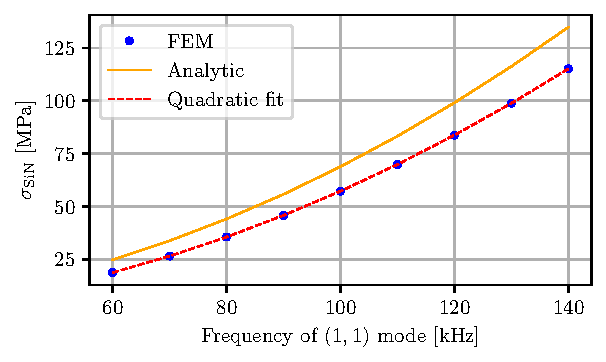
\includegraphics[]{figures/prestress_estimator.pdf}
    \caption{Prestress estimation using a quadratic fit to simulated data points. For comparison, the curve corresponding to the homogeneous-membrane approximation is shown.}
    \label{fig:prestress_estimator}
\end{figure}






\section{Implementation of Sampled Masses}
\label{sec:implementation_sampled_masses}

For the EMILIE device, two methods of sample deposition have been carried out \cite{timaracpopovic25}. The first is an aerosolization method, in which a gas is pumped through the perforation, resulting in aerosol deposition on the membrane \cite{Schmid13}. The second is nanoliter droplet dispensing, where a pre–mixed dispersion droplet containing nanoplastic particles is deposited on the membrane. After evaporation of the solvent, a residue of nanoplastic particles remains. Due to the coffee-ring effect \cite{MAMPALLIL18}, most of this residue accumulates along the rim of the droplet (see Figure \ref{fig:coffeering} (B)).

\begin{figure}[h]
    \centering
    \begin{overpic}[height=\domainheight,
    trim=2.2cm 2.2cm 2.2cm 2.2cm,
        clip]{figures/pngs/mesh_sampled.png}
        \put(10,90){\large\bfseries\textcolor{white}{A}}
    \end{overpic}%
    \hspace{1cm}
    \begin{overpic}[height=\domainheight]{figures/pngs/coffeering.png}
        \put(13,90){\large\bfseries\textcolor{white}{B}}
    \end{overpic}
    \caption{(\textbf{A}) Mesh for the simulation with default parameters and a region that resolves a coffee ring shaped sample. (\textbf{B}) Image of a sampled membrane with the formation of a coffee ring from a polystyrene solution droplet deposited on an EMILIE membrane.}
    \label{fig:coffeering}
\end{figure}


In this thesis, only the nanoliter droplet dispensing method is considered. However, a mass distribution resembling any other deposition technique could be implemented with minimal modification. In the following, we describe how the sampled mass has been modeled in the simulation.\\

Experimental results suggest that the sampled material itself exhibits a prestress, which can also be incorporated into the simulation. The simulation parameters \texttt{p} contain a Python dictionary \texttt{p["added\_masses"]}, which holds tuples of variables as listed in table \ref{tab:parameters}. Besides the self-explanatory parameters, there are:  
\texttt{coffee\_ring\_perctg}: the percentage of the sampled mass located in the coffee ring, with the remainder distributed inside the ring.  
\texttt{coffee\_prestress}: the prestress within the coffee ring.  
\texttt{non\_coffee\_prestress}: the prestress within the inner region.  

SEM images indicate that the prestress within the ring is low to negligible, since the nanoparticles are relatively far apart \cite{timaracpopovic25}.\\

If \texttt{p["added\_masses"]} is non-empty, the function \texttt{make\_geometry} adds nodes to the mesh along the coffee-ring boundaries. The function \texttt{generate\_sig\_fct} then sets the prestress values on and within the coffee ring, while \texttt{generate\_rho\_fct} defines the increased mass density according to the specified parameters. Finally, the function \texttt{force\_CF} incorporates the forcing term resulting from the prestress discontinuity at the coffee-ring boundary, as discussed in section \ref{sec:ela_pde}.\\

\section{Parameters}

This section summarizes the adaptable parameters of the simulation and their default values. In the implementation, the letter \texttt{p} is reserved for this set of parameters, stored in a Python dictionary. The adjustable parameters are listed in table \ref{tab:parameters}.  

Additional variables are computed internally from these input parameters. Default values can be initialized with the function \texttt{set\_p\_standard}.\\

\newpage 

\begin{table}[h]
    \centering
    \caption{Simulation parameters, their corresponding Python dictionary keys in \texttt{p}, descriptions, and default values. Parameters concerning added masses are stored in the dictionary \texttt{p["added\_masses"][i]}, where typically \texttt{i=0} since we consider only one coffee ring. Mesh- and algorithmic parameters are omitted.}
    \label{tab:parameters}
    \renewcommand{\arraystretch}{1.8}
    \begin{tabular}{llll}
        \textbf{Symbol} & \textbf{Python key} & \textbf{Description} & \textbf{Default value} \\
        \hline
        Materials&    &   &  \\
        $\sigma_\silnit,\sigma_\chro,\sigma_\gold$     & \texttt{"sigsin"}, \texttt{"sigcr"}, \texttt{"sigau"} & Prestress & \SI{24.7}{\mega\pascal}, \SI{1}{\giga\pascal}, \SI{40}{\mega\pascal}  \\
        $\rho_\silnit^\mathrm{3D},\rho_\chro^\mathrm{3D},\rho_\gold^\mathrm{3D}$  & \texttt{"rhosin"}, \texttt{"rhocr"}, \texttt{"rhoau"} & Densities (3D) & \SI{3440}{}, \SI{7140}{}, \SI{19320}{\kilogram\per\cubic\meter} \\
        $h_\silnit,h_\chro,h_\gold$  & \texttt{"hsin"}, \texttt{"hcr"}, \texttt{"hau"} & Thicknesses & \SI{50}{}, \SI{10}{}, \SI{90}{\nano\meter} \\
        $E_\silnit,\nu_\silnit$  & \texttt{"Esin"}, \texttt{"nu"} & Mechanical parameters & $\SI{250}{\giga\pascal}\cdot h_\silnit$, 0.23 \\
        Geometry&    &   &  \\
        $L$  & \texttt{"Lside"} & Membrane side length & \SI{1}{\milli\meter} \\
        $w_e$  & \texttt{"el\_width"} & Electrode width & \SI{10}{\micro\meter} \\
        $P_\mathrm{el}$  & \texttt{"rel\_max\_of\_electrode"} & See section \ref{sec:electrode_geometry} & \SI{0.9}{}\\
        $R_\mathrm{perf}$  & \texttt{"Rperf"} & Perforation radius & \SI{0.3}{\milli\meter}\\
        Perforation&    & Effective relative values & on perforation \\
        $\sigma_\mathbf{eff}^*$, $\rho_\mathbf{eff}^*$  & \texttt{"sigpercentage\_perf", "mper..."} & See section \ref{sec:definition_effective_parameters} & 1, 0.62 \\
        $E_\mathbf{eff}^*$  & \texttt{"Epercentage\_perf"} & & 0.362 \\
        $\nu_\mathbf{eff}^*$  & \texttt{"nupercentage\_perf"} & & 1.0 \\
        $\sigma_\mathbf{eff}^*-1$  & \texttt{"corr\_perf\_sig"} & & 0.0 \\
        Added masses &    &  &  \\
        $x_\mathrm{samp}, y_\mathrm{samp}$ & \texttt{"x\_coord"}, \texttt{"y\_coord"} & Coffee-ring center & $0.5, \SI{0.5}{\milli\meter}$ \\
        $m_\mathrm{samp}$ & \texttt{"mass"} & Sample mass & $0-\SI{40}{\nano\gram}$ \\
        $R_\mathrm{samp}$ & \texttt{"radius"} & Sample radius & \SI{0.25}{\milli\meter} \\
        & \texttt{"coffee\_ring\_perctg"} & See section \ref{sec:implementation_sampled_masses} & 0.8 \\
        $\sigma_\mathrm{samp}$& \texttt{"coffee\_prestress"} & See section \ref{sec:implementation_sampled_masses} & \SI{0}{\mega\pascal} \\
        $w_\mathrm{samp}$& \texttt{"coffee\_ring\_width"} & Ring width & \SI{5}{\micro\meter} \\
    \end{tabular}
\end{table}
\newpage









\section{Simulation with Timeout}

The PINVIT algorithm does not converge for every possible parameter set. Even with a maximum number of allowed iterations, the algorithm did not return in some cases. To address this, a wrapper with a timeout mechanism has been implemented. This functionality is provided in the wrapper function \texttt{solve\_wrapper} and the main function \texttt{solve\_with\_timeout}. A separate process running \texttt{solve\_wrapper} is instantiated using Python's \texttt{multiprocessing} library. For large simulation runs with a diverse set of parameters, this approach has proven highly convenient.  

Due to constraints on return values in the \texttt{multiprocessing} library, the \texttt{solve\_with\_timeout} function can return only the eigenvalues, but not the corresponding mode shapes. Therefore, for smaller runs where mode shapes are of interest, the regular \texttt{solve} function is still used.\\

\newpage
